\documentclass[12pt,journal,compsoc,onecolumn]{IEEEtran}
\usepackage{graphicx}
\usepackage{cite}
\usepackage{url}
\usepackage{caption}

\providecommand{\PSforPDF}[1]{#1}
\newcommand{\um} {$\mu$m}


\newcommand\MYhyperrefoptions{bookmarks=true,bookmarksnumbered=true,
pdfpagemode={UseOutlines},plainpages=false,pdfpagelabels=true,
colorlinks=true,linkcolor={black},citecolor={black},pagecolor={black},
urlcolor={black},
pdftitle={First interim report},%<!CHANGE!
pdfsubject={Typesetting},%<!CHANGE!
pdfauthor={Carsten Bruns \& Jakob Toft},%<!CHANGE!
pdfkeywords={High-speed communication, Voltage-mode driver, Low-power 10GB/s}}%<^!CHANGE!

% correct bad hyphenation here
\hyphenation{op-tical net-works semi-conduc-tor}

\usepackage[]{units}
\usepackage{graphicx}
\usepackage{subfigure}

\usepackage{epstopdf}

\usepackage{pgfplots} 
\usepgfplotslibrary{external}
\tikzexternalize

\usepackage{float}

\begin{document}
%
% paper title
% can use linebreaks \\ within to get better formatting as desired
\title{Design, Analysis and Simulation of an I/O Link\\Second interim report}

\author{Carsten Bruns
        \& Jakob Toft% <-this % stops a space

%\IEEEcompsoctitleabstractindextext{%
%\begin{abstract}
%\boldmath
%The abstract goes here.
%\end{abstract}


% Note that keywords are not normally used for peerreview papers.
\begin{IEEEkeywords}
High-Speed Data Links, Low-Power 10Gb/s link.
\end{IEEEkeywords}}


% make the title area
\maketitle

\IEEEdisplaynotcompsoctitleabstractindextext
\IEEEpeerreviewmaketitle


\section{Choice of the citcuit topology}

\IEEEPARstart{T}{odo} write sth here! \cite{cressler2007a}
\section{Transmitter schematics}

%TODO explain layering
%TODO explain sizing!! and give the values!

\begin{figure}[ht]
  \centering
  {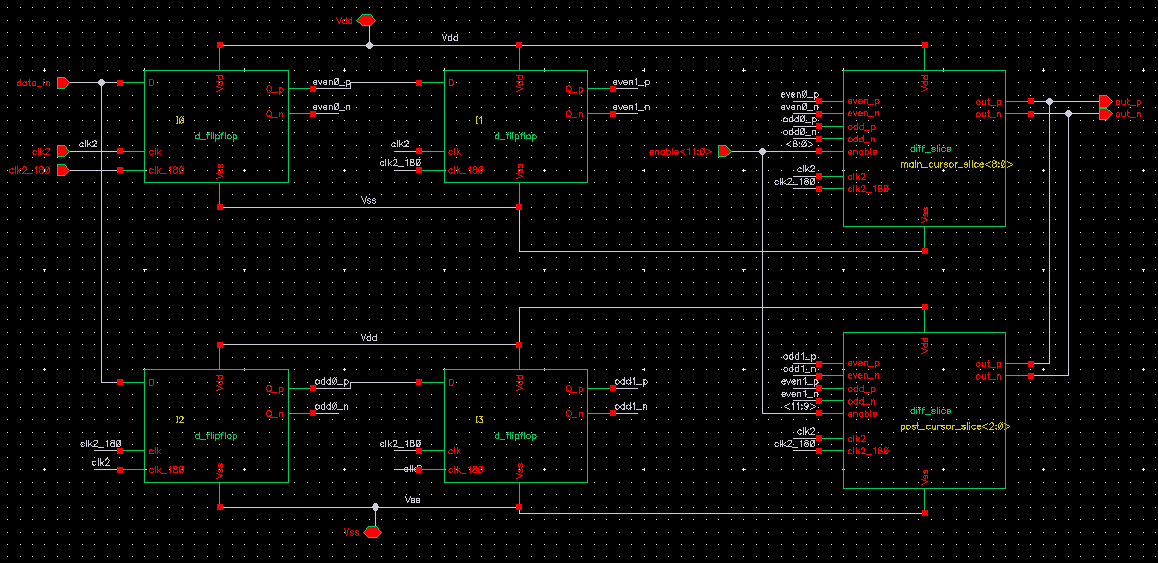
\includegraphics[scale=0.55]{img/transmitter.png}}
  \caption{Transmitter top level circuit}
  \label{fig:top_level}
\end{figure}

\begin{figure}[ht]
  \centering
  \subfigure[Differential slice]
  {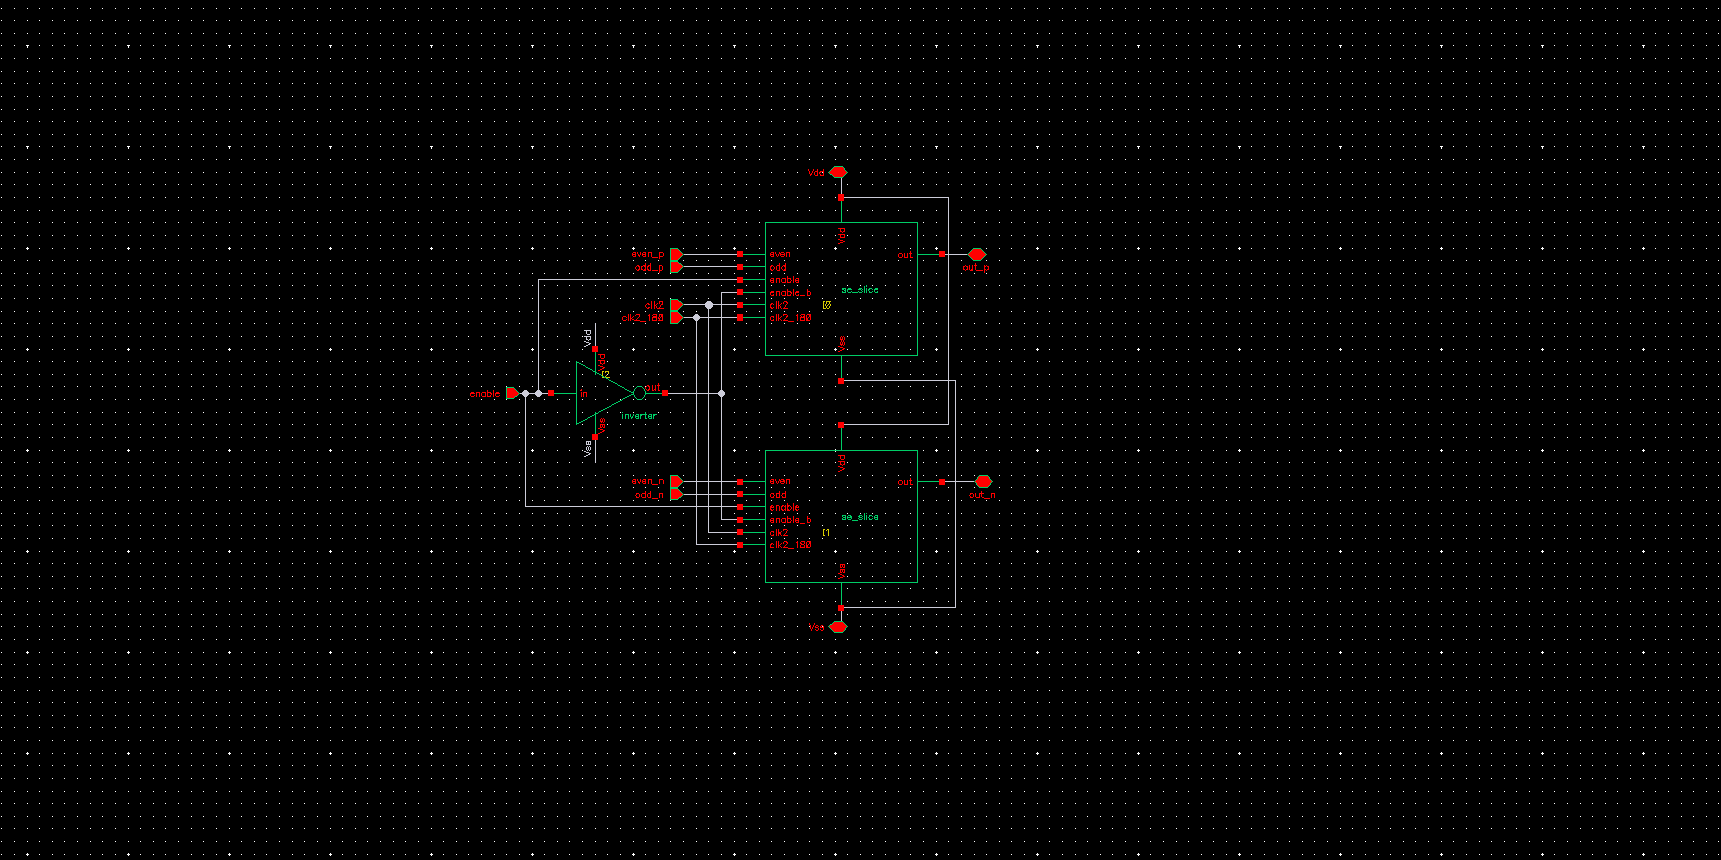
\includegraphics[scale=0.6]{img/diff_slice.png}}
  \subfigure[Single-ended slice]
  {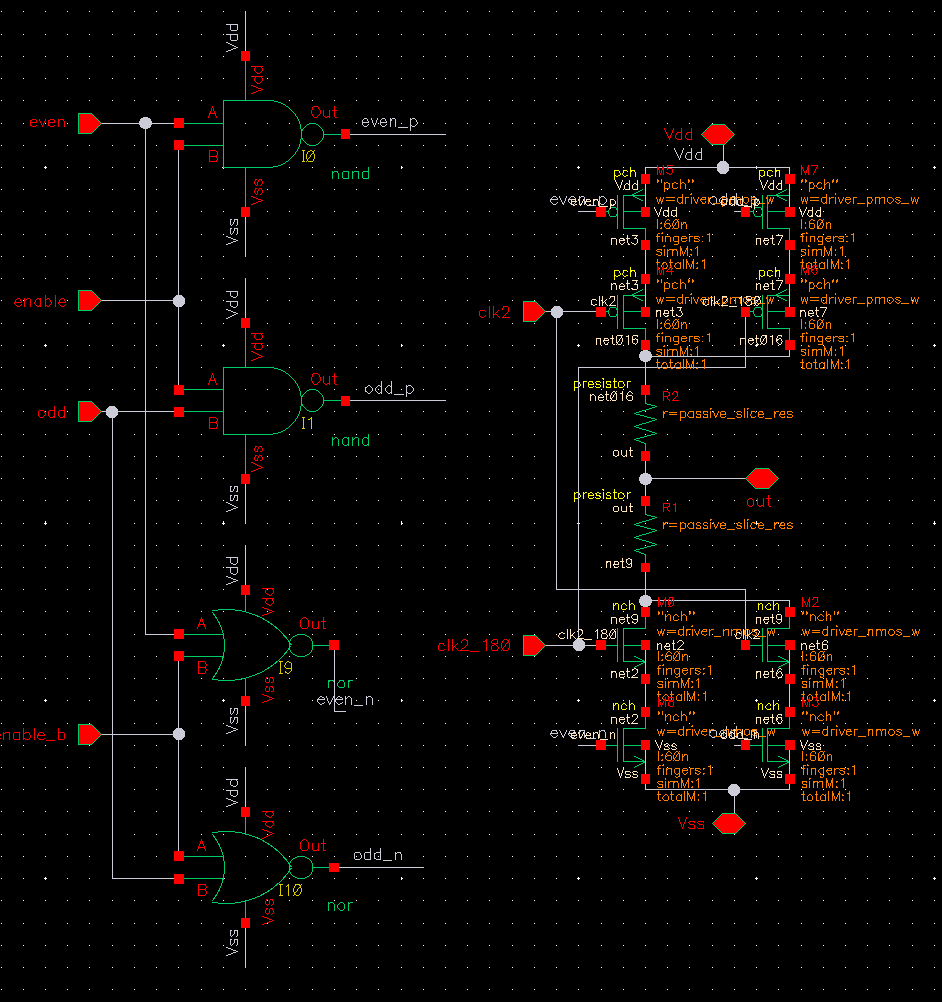
\includegraphics[scale=0.5]{img/se_slice.png}}
  \caption{Slice circuits}
  \label{fig:slices}
\end{figure}

\begin{figure}[ht]
  \centering
  {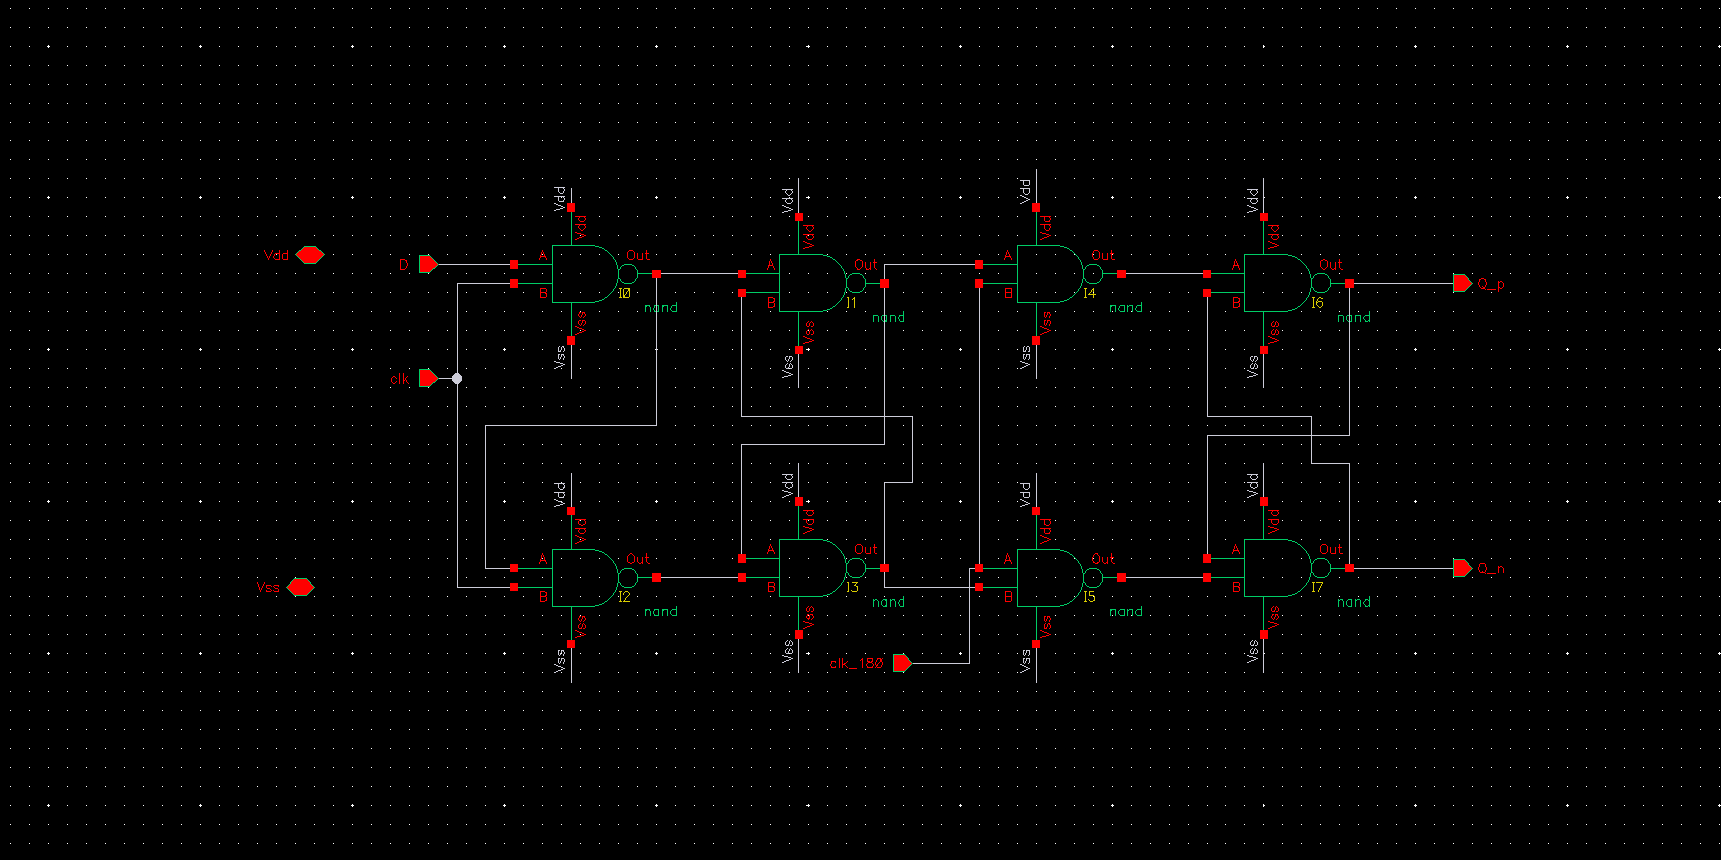
\includegraphics[scale=0.47]{img/flipflop.png}}
  \caption{D-Flipflop}
  \label{fig:flipflop}
\end{figure}

\begin{figure}[ht]
  \centering
  \subfigure[Inverter]
  {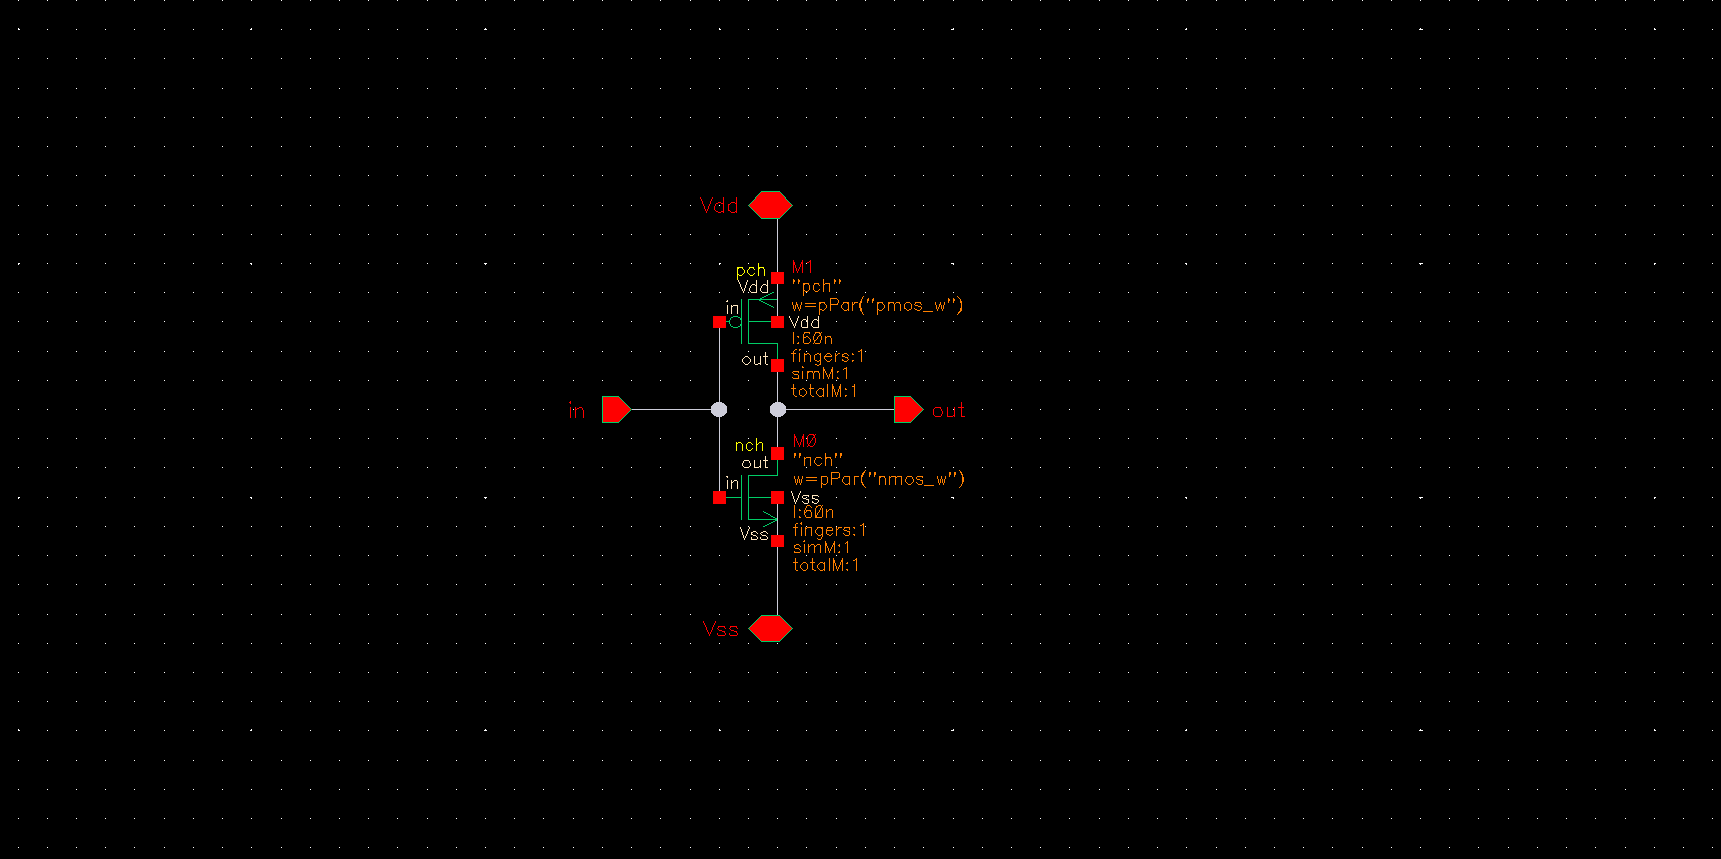
\includegraphics[scale=0.5]{img/inverter.png}}
  \subfigure[NAND gate]
  {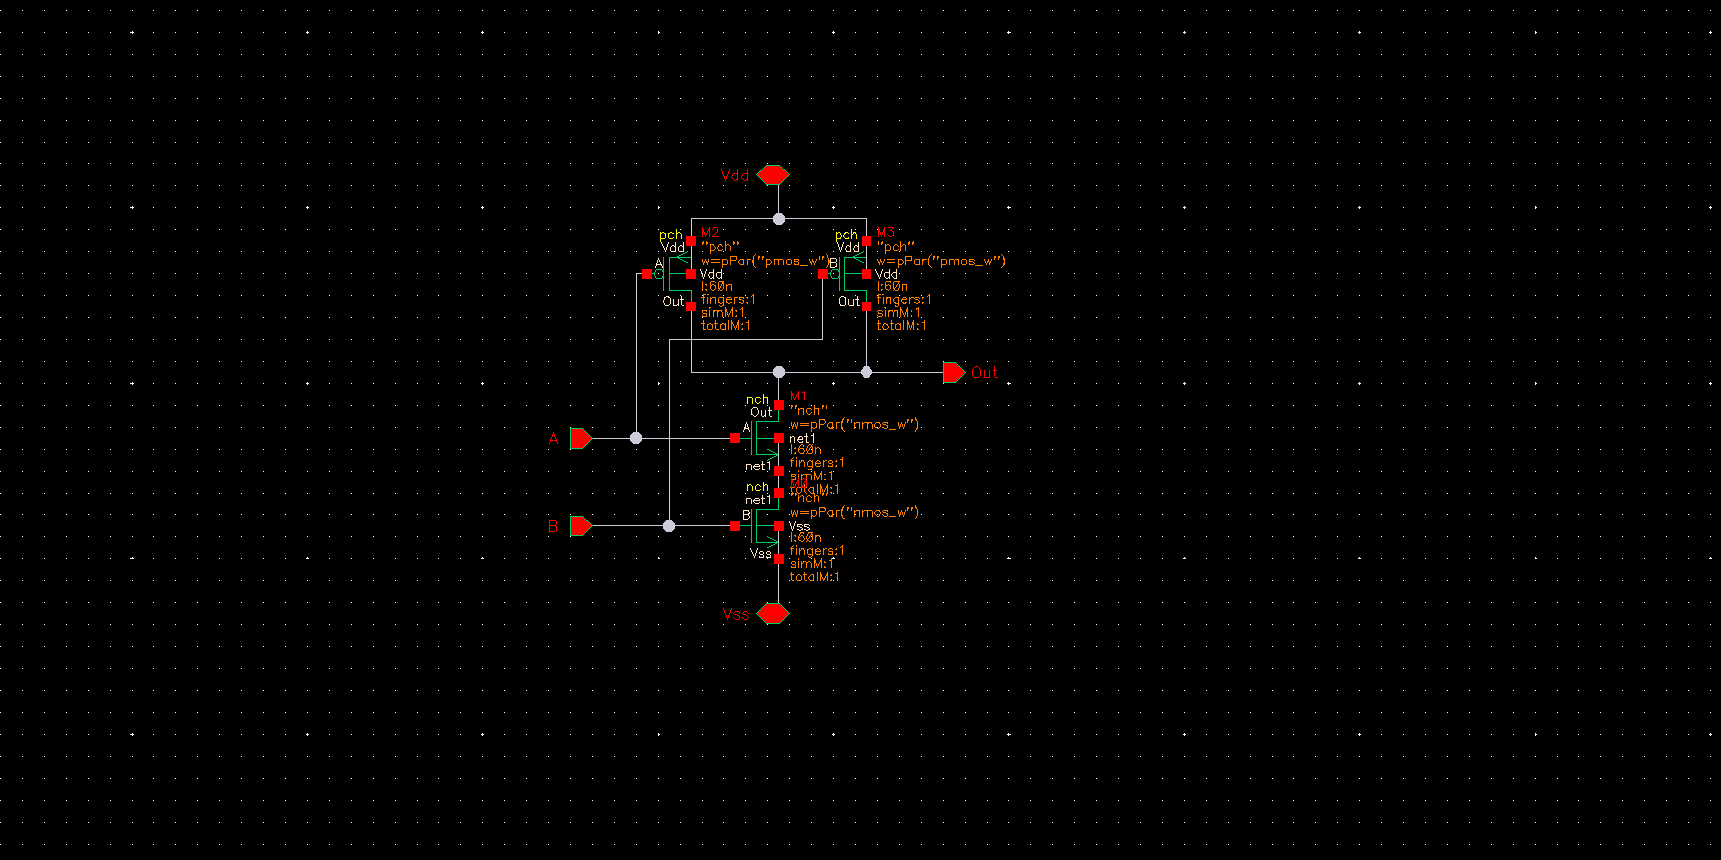
\includegraphics[scale=0.5]{img/nand.png}}
  \subfigure[NOR gate]
  {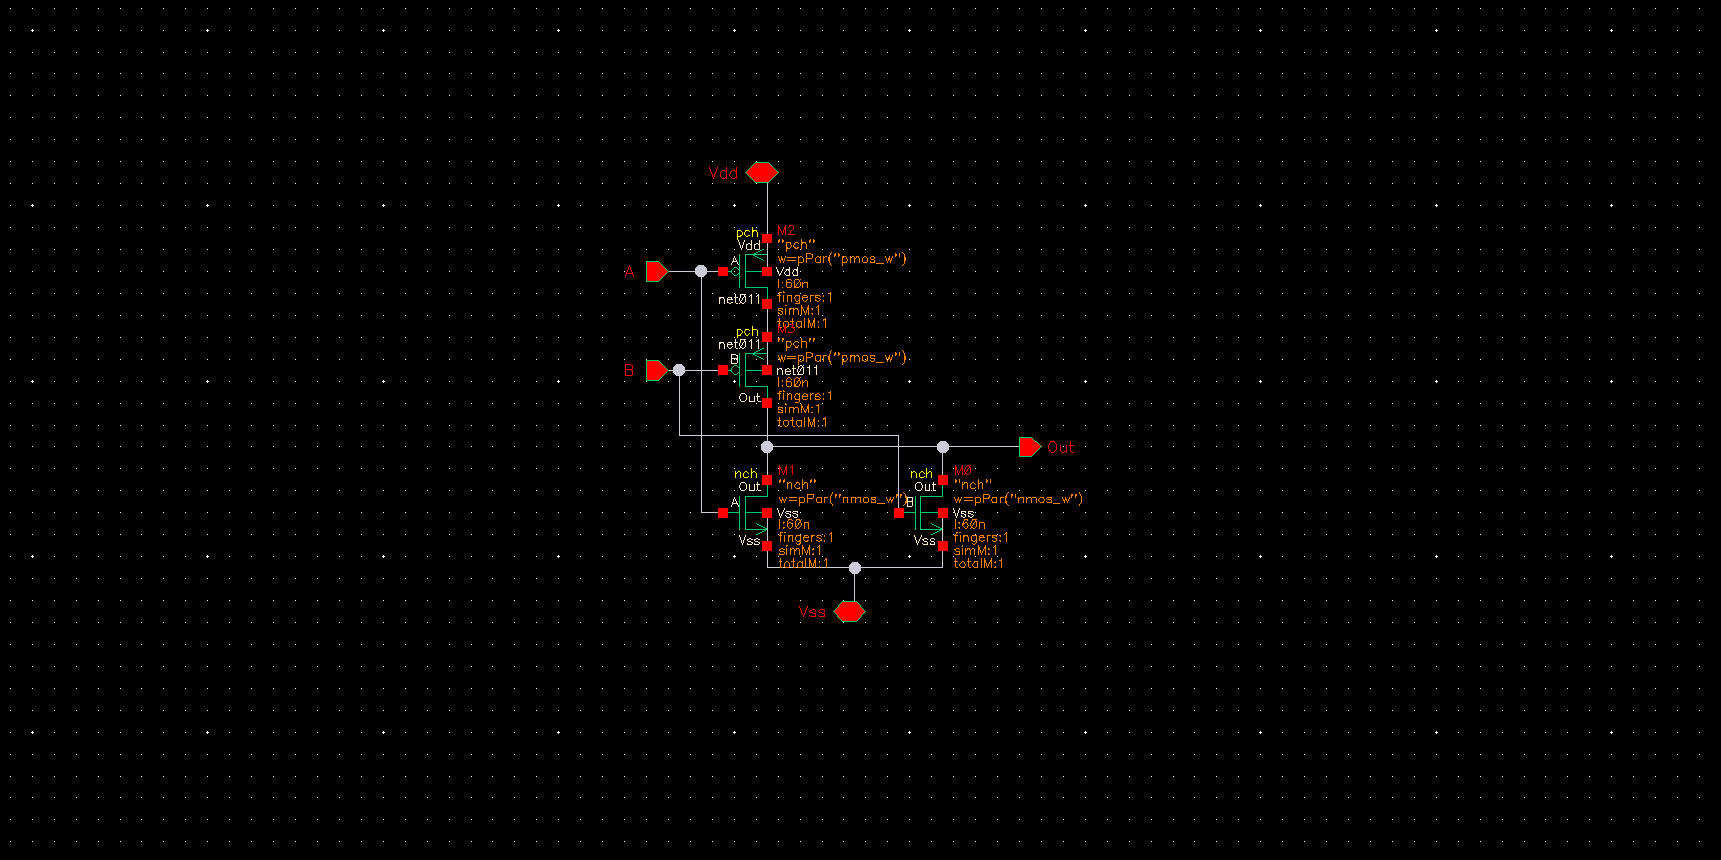
\includegraphics[scale=0.5]{img/nor.png}}
  \caption{Simple gate circuits}
  \label{fig:gates}
\end{figure}
\section{Output signals for different input signals}

\IEEEPARstart{T}{odo} write sth here!

%TODO alternating 6UI
%TODO eye PRBS15, 10,000UI
%TODO wc eye
\section{Impedance tuning}

\IEEEPARstart{T}{odo} write sth here!

%TODO tuning range graph
\subsection{Power consumption}
The power consumption at \unit[10]{Gb/s} PRBS15 data and \unit[1]{V} power supply as well as at \unit[2]{Gb/s} and \unit[0.7]{V} power supply is shown in table \ref{tab:power_consumption_rx}. The complete receiver consists of two receiver slices, each of them of VOA, strongARM and RS-FlipFlop (see section \ref{sec:rx_schematics}).

\begin{table}[H] %TODO add values for 2GB/s 0.7V
  \centering
  \begin{tabular}{l|l|l}
    component & \unit[10]{Gb/s} at \unit[1]{V} & \unit[2]{Gb/s} at \unit[0.7]{V}\\
    \hline
    complete receiver & \unit[2217]{\uW} & \unit[223]{\uW}\\
    clock buffers & \unit[1888]{\uW} & \unit[171]{\uW}\\
    receiver slice & \unit[164,67]{\uW} & \unit[25,92]{\uW}\\
    VOA & \unit[49,54]{\uW} & \unit[14,73]{\uW}\\
    strongARM & \unit[42,27]{\uW} & \unit[3,718]{\uW}\\
    RS-FlipFlop & \unit[72,86]{\uW} & \unit[7,471]{\uW}\\
  \end{tabular}
  \caption{Receiver power consumption with PRBS15 data}
  \label{tab:power_consumption_rx}
\end{table}

As it can be observed the total power consumption of the receiver is 2.217mA, which at 1V gives a power consumption of 2.217mW, resulting in a energy consumption of 2.217mJ per second. This gives that the energy per bit is 0.2217 pJ per bit, it seems like the power consumption of receiver is pretty decent and that future work, in reducing power consumption of the link, should be done on the transmitter.
%\section{Performance results}

\IEEEPARstart{T}{odo} write sth here!

%TODO table with performance/specs



% Can use something like this to put references on a page
% by themselves when using endfloat and the captionsoff option.
\ifCLASSOPTIONcaptionsoff
  \newpage
\fi

\newpage
\section{Bibliography}
\bibliography{biblio}{}
\bibliographystyle{plain}


\end{document}


